\documentclass[14pt]{extbook}
\usepackage{multicol, enumerate, enumitem, hyperref, color, soul, setspace, parskip, fancyhdr} %General Packages
\usepackage{amssymb, amsthm, amsmath, latexsym, units, mathtools} %Math Packages
\everymath{\displaystyle} %All math in Display Style
% Packages with additional options
\usepackage[headsep=0.5cm,headheight=12pt, left=1 in,right= 1 in,top= 1 in,bottom= 1 in]{geometry}
\usepackage[usenames,dvipsnames]{xcolor}
\usepackage{dashrule}  % Package to use the command below to create lines between items
\newcommand{\litem}[1]{\item#1\hspace*{-1cm}\rule{\textwidth}{0.4pt}}
\pagestyle{fancy}
\lhead{Makeup Progress Quiz 2}
\chead{}
\rhead{Version A}
\lfoot{5763-3522}
\cfoot{}
\rfoot{Spring 2021}
\begin{document}

\begin{enumerate}
\litem{
Determine the horizontal and/or oblique asymptotes in the rational function below.\[ f(x) = \frac{9x^{3} +12 x^{2} -17 x -20}{3x^{2} +8 x -16} \]\begin{enumerate}[label=\Alph*.]
\item \( \text{Oblique Asymptote of } y = 3x -4. \)
\item \( \text{Horizontal Asymptote of } y = 3.0 \text{ and Oblique Asymptote of } y = 3x -4 \)
\item \( \text{Horizontal Asymptote of } y = 3.0  \)
\item \( \text{Horizontal Asymptote at } y = -4.0 \)
\item \( \text{Horizontal Asymptote of } y = -4.0 \text{ and Oblique Asymptote of } y = 3x -4 \)

\end{enumerate} }
\litem{
Determine the vertical asymptotes and holes in the rational function below.\[ f(x) = \frac{16x^{3} +16 x^{2} -25 x -25}{12x^{2} -7 x -10} \]\begin{enumerate}[label=\Alph*.]
\item \( \text{Vertical Asymptote of } x = 1.333 \text{ and hole at } x = 1.25 \)
\item \( \text{Vertical Asymptote of } x = -0.667 \text{ and hole at } x = 1.25 \)
\item \( \text{Vertical Asymptotes of } x = -0.667 \text{ and } x = -1.25 \text{ with a hole at } x = 1.25 \)
\item \( \text{Vertical Asymptotes of } x = -0.667 \text{ and } x = 1.25 \text{ with no holes.} \)
\item \( \text{Holes at } x = -0.667 \text{ and } x = 1.25 \text{ with no vertical asymptotes.} \)

\end{enumerate} }
\litem{
Which of the following functions \textit{could} be the graph below?
\begin{center}
    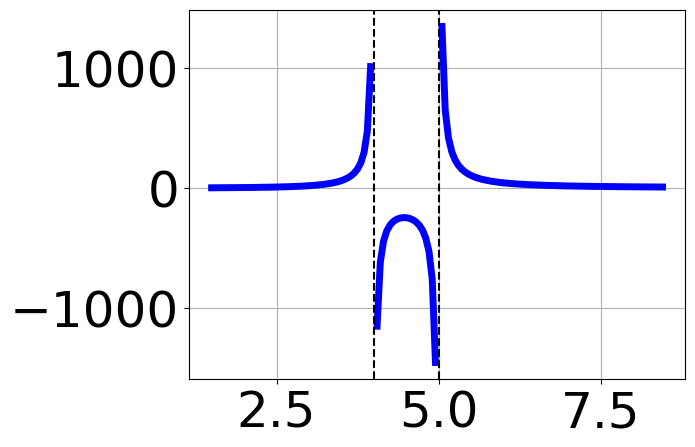
\includegraphics[width=0.5\textwidth]{../Figures/identifyGraphOfRationalFunctionCopyA.png}
\end{center}
\begin{enumerate}[label=\Alph*.]
\item \( f(x)=\frac{x^{3} +8 x^{2} +17 x + 10}{x^{3} -15 x^{2} +74 x -120} \)
\item \( f(x)=\frac{x^{3} -1 x^{2} -32 x + 60}{x^{3} +15 x^{2} +74 x + 120} \)
\item \( f(x)=\frac{x^{3} -1 x^{2} -32 x + 60}{x^{3} +15 x^{2} +74 x + 120} \)
\item \( f(x)=\frac{x^{3} + x^{2} -32 x -60}{x^{3} -15 x^{2} +74 x -120} \)
\item \( \text{None of the above are possible equations for the graph.} \)

\end{enumerate} }
\litem{
Determine the horizontal and/or oblique asymptotes in the rational function below.\[ f(x) = \frac{12x^{3} +53 x^{2} -5 x -100}{3x^{2} -x -10} \]\begin{enumerate}[label=\Alph*.]
\item \( \text{Horizontal Asymptote of } y = 4.0 \text{ and Oblique Asymptote of } y = 4x + 19 \)
\item \( \text{Horizontal Asymptote at } y = 2.0 \)
\item \( \text{Horizontal Asymptote of } y = 4.0  \)
\item \( \text{Oblique Asymptote of } y = 4x + 19. \)
\item \( \text{Horizontal Asymptote of } y = 2.0 \text{ and Oblique Asymptote of } y = 4x + 19 \)

\end{enumerate} }
\litem{
Determine the vertical asymptotes and holes in the rational function below.\[ f(x) = \frac{12x^{3} -19 x^{2} -45 x -18}{12x^{2} +x -6} \]\begin{enumerate}[label=\Alph*.]
\item \( \text{Vertical Asymptotes of } x = 0.667 \text{ and } x = -0.667 \text{ with a hole at } x = -0.75 \)
\item \( \text{Vertical Asymptote of } x = 1.0 \text{ and hole at } x = -0.75 \)
\item \( \text{Holes at } x = 0.667 \text{ and } x = -0.75 \text{ with no vertical asymptotes.} \)
\item \( \text{Vertical Asymptotes of } x = 0.667 \text{ and } x = -0.75 \text{ with no holes.} \)
\item \( \text{Vertical Asymptote of } x = 0.667 \text{ and hole at } x = -0.75 \)

\end{enumerate} }
\litem{
Determine the horizontal and/or oblique asymptotes in the rational function below.\[ f(x) = \frac{12x^{3} +55 x^{2} +18 x -40}{6x^{3} +4 x^{2} +24 x -32} \]\begin{enumerate}[label=\Alph*.]
\item \( \text{Horizontal Asymptote of } y = 2.000  \)
\item \( \text{Vertical Asymptote of } y = -4  \)
\item \( \text{Horizontal Asymptote of } y = 0  \)
\item \( \text{None of the above} \)
\item \( \text{Vertical Asymptote of } y = -2.000  \)

\end{enumerate} }
\litem{
Determine the vertical asymptotes and holes in the rational function below.\[ f(x) = \frac{4x^{3} -32 x^{2} +79 x -60}{6x^{2} -17 x + 12} \]\begin{enumerate}[label=\Alph*.]
\item \( \text{Vertical Asymptotes of } x = 1.333 \text{ and } x = 2.5 \text{ with a hole at } x = 1.5 \)
\item \( \text{Vertical Asymptote of } x = 1.333 \text{ and hole at } x = 1.5 \)
\item \( \text{Holes at } x = 1.333 \text{ and } x = 1.5 \text{ with no vertical asymptotes.} \)
\item \( \text{Vertical Asymptote of } x = 0.667 \text{ and hole at } x = 1.5 \)
\item \( \text{Vertical Asymptotes of } x = 1.333 \text{ and } x = 1.5 \text{ with no holes.} \)

\end{enumerate} }
\litem{
Determine the vertical asymptotes and holes in the rational function below.\[ f(x) = \frac{12x^{3} +13 x^{2} -37 x -30}{6x^{2} -19 x + 15} \]\begin{enumerate}[label=\Alph*.]
\item \( \text{Vertical Asymptotes of } x = 1.5 \text{ and } x = 1.667 \text{ with no holes.} \)
\item \( \text{Holes at } x = 1.5 \text{ and } x = 1.667 \text{ with no vertical asymptotes.} \)
\item \( \text{Vertical Asymptotes of } x = 1.5 \text{ and } x = -0.75 \text{ with a hole at } x = 1.667 \)
\item \( \text{Vertical Asymptote of } x = 2.0 \text{ and hole at } x = 1.667 \)
\item \( \text{Vertical Asymptote of } x = 1.5 \text{ and hole at } x = 1.667 \)

\end{enumerate} }
\litem{
Which of the following functions \textit{could} be the graph below?
\begin{center}
    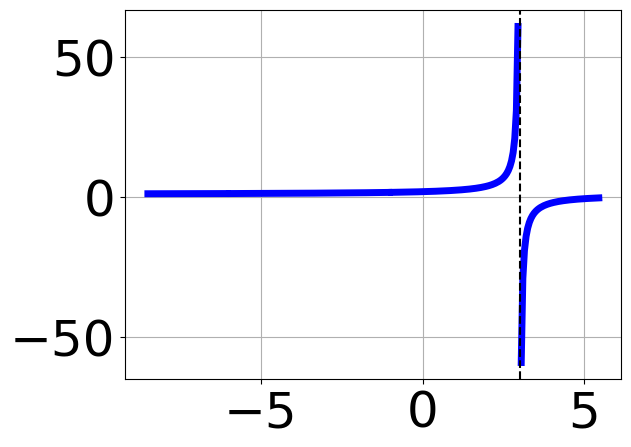
\includegraphics[width=0.5\textwidth]{../Figures/identifyGraphOfRationalFunctionA.png}
\end{center}
\begin{enumerate}[label=\Alph*.]
\item \( f(x)=\frac{x^{3} -1 x^{2} -36 x + 36}{x^{3} -4 x^{2} -15 x + 18} \)
\item \( f(x)=\frac{x^{3} -1 x^{2} -36 x + 36}{x^{3} -4 x^{2} -15 x + 18} \)
\item \( f(x)=\frac{x^{3} -8 x^{2} +4 x + 48}{x^{3} +4 x^{2} -15 x -18} \)
\item \( f(x)=\frac{x^{3} + x^{2} -36 x -36}{x^{3} +4 x^{2} -15 x -18} \)
\item \( \text{None of the above are possible equations for the graph.} \)

\end{enumerate} }
\litem{
Determine the horizontal and/or oblique asymptotes in the rational function below.\[ f(x) = \frac{12x^{3} -47 x^{2} +56 x -20}{4x^{3} +2 x^{2} -29 x + 30} \]\begin{enumerate}[label=\Alph*.]
\item \( \text{Vertical Asymptote of } y = -3.000  \)
\item \( \text{Vertical Asymptote of } y = 2  \)
\item \( \text{None of the above} \)
\item \( \text{Horizontal Asymptote of } y = 3.000  \)
\item \( \text{Horizontal Asymptote of } y = 0  \)

\end{enumerate} }
\end{enumerate}

\end{document}